\documentclass[12pt,a4paper]{ctexart}

\usepackage[left=2.2cm,right=2.2cm,top=2.5cm,bottom=2.5cm]{geometry}
\usepackage{graphicx}
\usepackage{xcolor}
\usepackage[most]{tcolorbox}
\usepackage{setspace}
\usepackage{hyperref}
\usepackage{amsmath}
\usepackage{float}
\usepackage{xeCJK}      % 如果你使用中文，需要这个宏包（如果文档类是ctexart则不需要）
\usepackage{booktabs}   % 用于绘制三线表（\toprule, \midrule, \bottomrule）
\usepackage{multirow}   % 用于处理纵向合并的单元格
\usepackage{tabularx}
\usepackage{placeins}

\pagestyle{empty}
\setlength{\parindent}{2em}
\setlength{\parskip}{0.5em}
\linespread{1.35}

\definecolor{linegray}{RGB}{190,190,190}
\definecolor{textgray}{RGB}{110,110,110}

\newcommand{\templaterule}{
  \noindent\color{linegray}\rule{\textwidth}{0.5pt}\color{black}
}


\begin{document}

{\zihao{2} 课程项目期中进度报告\par}

\vspace{1em}
\templaterule
\vspace{1.5em}

{\zihao{3}\bfseries 《多媒体信息处理》2026 春季学期\par}
\vspace{1em}

\begin{tcolorbox}[
  enhanced,
  breakable,
  colback=white,
  colframe=white,
  boxrule=0pt,
  left=1em,
  right=0pt,
  top=0.5em,
  bottom=0.5em,
  borderline west={1.2pt}{0pt}{linegray}
]
\noindent
\textbf{项目名称：} 视网膜光凝手术智能教学游戏系统\\
\textbf{小组成员：} 冯俊铭、吴嘉淇、林鸿渝、陈俊希、吴雨潼、史卓然\\
\textbf{指导教师：} 刘江老师\\
\textbf{提交日期：} 2026年4月18日

\end{tcolorbox}

\templaterule

\section{项目概述}
本项目属于教育类游戏的模拟子类，面向真实眼底外科手术医师、相关从业者以及对眼科知识感兴趣的玩家。设计初衷在于教授眼科医生眼底光凝术以及相关病症诊断。基于面向对象的小众与专业性质，项目在设计层面便考虑最大化真实性与严谨性，在此基础上尽可能丰富游玩的视听体验，辅佐小权重的娱乐内容。最后使得玩家在获得“学会眼底光凝术”本身的教育快乐的同时，也体验到绝不枯燥的游戏内容体验。

游戏核心内容在于光凝术诊断与治疗的全流程。玩家在游戏中，会经营一家私人诊所，扮演眼底光凝术手术医师，不断经历“接取任务-线上问诊-手术执行-术后评估”的循环，以获得愈发高超的光凝术相关技能。与此同时，根据玩家近期诊疗表现与病症难度，动态调整病症派发类别与难度，辅佐“成就”与游戏内经济，实现玩家持续纠错保优，或逐步“挑战自我”的心流正向循环，不断激励玩家游玩。

对于“接取任务-线上问诊-手术执行-术后评估”的核心流程，游戏最终以游戏内短信交流、手术视野与光斑模拟以及图鉴式全流程图文复盘的形式进行呈现。具体而言，通过基于后端大模型的提示词工程，将医学文本病历与病症无关病征进行组合，以日常口语形式，在手机聊天窗口向玩家提供病症与光凝术需求判断所需的文本与图像依据，实现模拟线上问诊，以及提高医生病症判断水平的目的；游戏中内置完整的光凝手术模拟程序，确保医生能够提前熟悉真实手术环境，提高临床环境下的适应与实操能力；游戏内的智能评价系统模块则通过从题库中读取样本的标准答案、和从游戏程序获得玩家的操作日志，从位置与范围、强度与能量、密度与均匀度三个维度进行评分计算，最后将计算好的玩家得分、当前题目对应的病历文本、以及从专家知识库中获取相关专业知识整理后输入大语言模型(LLM)，得到完整的、带有专业医学建议的教学评估报告，以给予玩家实时的教学反馈。

\begin{figure}[h]
    \centering
    \includegraphics[width=1\linewidth]{f1.png}
    \caption{游戏开始页面}
    \label{fig:placeholder}
\end{figure}

\section{多媒体数据定义}

本项目针对视网膜光凝手术的仿真教学需求，主要集成了六大模态中图像、文本、图形、动画及语音几种模态的数据。

\begin{itemize}
    \item \textbf{图像模态}：包含由欧堡（Optos）超广角相机拍摄的伪彩图以及蔡司（Zeiss）眼底图，涵盖术前诊断、术后即刻及两周随访等关键时间节点。此外，还涉及用于智能评价的特征图，如视网膜大血管分割掩码、黄斑中心凹及视盘区域的危险区掩码。
    \item \textbf{文本与结构化数据}：包含非结构化的患者主诉病历及临床诊断文本，以及高度结构化的 JSON 数据。JSON 数据详细定义了题库层的标准参数、靶区多边形坐标，以及实时记录玩家操作的日志，包括每个光斑的 ID、功率、曝光时间、空间坐标及是否为试打状态等。
    \item \textbf{图形与动画模态}：系统采用像素风格构建诊疗室中枢场景。动画部分实现了玩家在行走、操作光凝仪、查阅文档以及微波炉交互等动作间的平滑切换。同时，图形模态还包括基于物理公式实时渲染的激光光斑，能够细腻呈现不同能量等级下的视网膜热损伤视觉效果。
    \item \textbf{语音模态}：包含环境背景音乐、诊疗室设备交互音效以及手术执行时的物理反馈声。通过视听结合的方式，为玩家提供实时的操作反馈，增强临床模拟的临场感。
\end{itemize}

\section{系统架构与技术路线}

\subsection{四层智能教学架构}

系统采用分层设计以支持关卡生成,手术模拟与智能反馈的核心游玩流程：
\begin{figure}[h]
    \centering
    \begin{minipage}{0.48\linewidth}
        \centering
        \includegraphics[width=\linewidth]{f2.png}
        \caption{系统架构图}
        \label{fig:sys_arch}
    \end{minipage}
    \hfill % 在两个 minipage 之间填充弹性间距
    \begin{minipage}{0.48\linewidth}
        \centering
        \includegraphics[width=\linewidth]{f3.png}
        \caption{数据流动图}
        \label{fig:data_flow}
    \end{minipage}
\end{figure}
\begin{enumerate}
    \item \textbf{题库层}：存储术前图、病历、标准手术参数及危险区掩码。
    \item \textbf{关卡生成层}：通过生成式模型根据题库数据动态构建游戏场景。
    \item \textbf{手术仿真层}：基于游戏引擎实现参数控制台、物理仿真渲染及玩家操作记录。
    \item \textbf{教学复盘层}：利用大语言模型（LLM）结合专家知识库，将结构化评分转化为自然语言报告。
\end{enumerate}

\subsection{核心技术与算法总结}

\subsubsection{基于 Unity 的诊疗场景搭建与交互组织}

为承载光凝术诊断与治疗全流程中的任务接取、术前判断、术后复盘与页面调度，本项目采用 Unity 进行前端场景搭建与交互逻辑组织。相较于静态界面堆叠方案，Unity 在场景切换、角色控制、UI 动画、脚本驱动数据绑定等方面具有更高的实现灵活性，能够较好支持本项目“接取任务--线上问诊--手术执行--术后评估”的循环式体验设计。基于此，我们将非手术部分的关键前端内容划分为术前任务接取与线上问诊场景、术后图鉴式复盘反馈场景，以及作为统一调度入口的诊所中枢场景三部分，并通过脚本实现三者之间的跳转、数据传递与交互协调。

\paragraph{术前任务接取与线上问诊场景}

术前任务接取与线上问诊界面如图~\ref{fig:unity_phone_consult} 所示。该部分以“游戏内手机”为统一入口，将系统派发的任务组织为联系人列表项，呈现在左侧栏中。每个任务联系人均包含头像和备注信息预览，以模拟现实移动端聊天软件的交互习惯，降低玩家的认知切换成本。玩家点击对应联系人后，右侧聊天窗口会动态加载该患者的问诊内容，并展示患者发送的文本信息与术前眼底图像。


在信息设计上，我们将问诊依据拆分为两类：其一为医院侧提供的结构化文本病例与术前眼底图像，作为病症判断的直接证据；其二为患者侧以聊天文本形式给出的口语化病情描述，其中不仅包含与病症高度相关的症状表述，也预留了与医学判断弱相关甚至无关的生活化干扰信息，以更贴近真实线上问诊情境。

从 Unity 实现角度看，该页面采用“左侧联系人滚动列表 + 右侧聊天内容面板”的双栏布局，通过脚本进行联系人点击事件监听、聊天内容容器的动态刷新、患者图像消息与文本消息的差异化渲染，以及按钮驱动的诊疗意图选择。该设计使得任务接取不再是单纯的菜单跳转，而是被包装为诊前信息接收与解释过程，有助于玩家建立“先问诊、后判断、再决定是否实施光凝术”的临床流程意识。

\begin{figure}
    \centering
    \includegraphics[width=1\linewidth]{unity_phone_consult.png}
    \caption{游戏内手机与聊天界面}
    \label{fig:unity_phone_consult}
\end{figure}

\paragraph{术后图鉴式复盘反馈场景}

术后复盘反馈界面如图~\ref{fig:unity_postop_report} 所示。该页面采用图鉴式双页结构，以“左页记录诊前依据，右页记录诊后反馈”为基本组织逻辑，辅助玩家在一次诊疗结束后对全过程进行系统复盘。左侧页面主要记录玩家术前对病症的诊断结果以及是否实施光凝术的判断，同时保留其作出判断时所依据的关键信息，包括关键文本病例与术前眼底图像，从而保证玩家在阅读术后反馈时能够回溯自身决策来源，而非仅被动接受结果。

右侧页面进一步划分为上下两个信息区域。右上部分展示病灶区域的局部截图，用于并列对比标准答案打点分布与玩家实际打点策略，以直观呈现两者在病灶覆盖、打点形态与病灶边界控制方面的差异。页面中设置眼状按钮，点击后可弹出参数面板，以更细粒度地展示标准方案与玩家方案在参数设置上的差异，包括但不限于光斑大小、曝光时长、参数组合与打点策略等内容，从而帮助玩家由“结果差异”进一步追溯至“操作原因”。

右下部分则承载系统对于玩家诊疗全过程的分析反馈，内容上划分为优点、缺点与改进建议三个维度。优点部分强调本次操作中保留价值较高的策略与行为模式，防止玩家因单次失误而忽略已有正确操作；缺点部分指出当前诊疗中的关键失分点或风险点；改进建议部分则尝试将系统评估结果转译为可执行的后续调优方向，帮助玩家形成基于反馈的闭环修正。整体而言，该页面不仅承担“结果展示”功能，更承担“行为解释”与“学习矫正”功能。

\begin{figure}
    \centering
    \includegraphics[width=1\linewidth]{unity_postop_report.png}
    \caption{图鉴式诊疗全程图文反馈报告}
    \label{fig:unity_postop_report}
\end{figure}

\paragraph{诊所中枢场景与页面调度}

诊所中枢场景如图~\ref{fig:unity_clinic_hub} 所示，是本项目中除手术场景外最核心的页面调度中心。玩家在该场景中扮演经营私人诊所的光凝术医师，通过角色左右移动与特定物体交互，实现不同功能页面与场景之间的切换。具体而言，玩家可在诊所环境中与电脑、光凝仪、微波炉、文档柜等物体发生交互，其中手机问诊界面同样由该中枢场景呼出。这样一来，原本分散的任务入口被统一收束到诊所经营这一叙事空间中，有助于增强各功能模块之间的语义连贯性。

\begin{figure}
    \centering
    \includegraphics[width=1\linewidth]{unity_clinic.png}
    \caption{诊疗室场景与碰撞检测示意}
    \label{fig:unity_clinic_hub}
\end{figure}

从实现机制上看，中枢场景依赖 Unity 的 2D 场景搭建能力、碰撞检测机制与脚本驱动交互逻辑来组织页面跳转。角色在场景内以左右移动为主，通过触发交互检测区域并按下交互键完成行为确认；系统根据当前交互对象类型，进一步执行页面打开、场景切换、UI 覆盖层播放或数据记录调取等逻辑。该设计在工程上形成了较清晰的“场景--交互对象--目标页面”映射关系，使得功能扩展时只需新增交互点与对应逻辑，而不必频繁重构整体页面体系。

\subsubsection{光斑凝手术模拟}

\paragraph{光斑等级公式}

在本项目中，光凝手术模拟任务主要被划分为公式建模、图形渲染以及 Unity 场景搭建三个子任务。

在光斑等级公式的建模时，我参考了Jain 等人$^1$ 关于脉冲持续时间对视网膜光凝病变影响的研究。在该项研究中，定量实验表明视网膜病变直径与激光功率呈线性增长关系，而与脉冲持续时间呈对数增长关系。基于上述定量指标，并结合热扩散规律及面积对能量的衰减作用，本项目将光凝热作用公式设定为：
\begin{equation}
z = \ln\left(\frac{t}{t_0}\right) + \beta k_{\mathrm{color}} \left(\frac{P}{P_0}\right) \left(\frac{d_0}{d}\right)^{\gamma} \left(1-e^{-\frac{t/1000}{\tau_s}}\right)
\end{equation}
在该模型中，$P$、$t$、$d$ 分别代表功率、时间和光斑直径，$k_{\mathrm{color}}$ 则是针对不同波长激光的经验系数。公式设计确保了功率增大、曝光时间延长或光斑缩小均能增强热作用效应。

算法的核心流程是通过蒙特卡洛空间采样结合随机搜索算法对公式参数进行全局寻优。首先，在 $50 \sim 500$ 的参数空间内进行大规模随机采样，利用 L-BFGS-B 优化器对初始参数进行迭代。该过程依靠蒙特卡洛算法生成的点云进行空间覆盖，之后采用启发式搜索快速收敛至最优解。

约束机制分为三个层面。首先是硬约束，要求固定实验数据点的计算结果必须严格落在目标等级（如 2 级或 3 级）的阈值区间内，并满足设定的安全边距。其次是软约束，在范围约束的中心点周围生成采样点云，通过最小化点云偏离目标的概率来增强决策边界的鲁棒性。最后是单调性约束，由于临床上的不确定性，我在数据预处理阶段清洗掉了不符合“参数更强则等级更高”逻辑的可疑数据点，确保模型符合基本的生物先验知识。

拟合所采用的代价函数由四部分加权组成。其一为硬约束惩罚，利用 Softplus 函数构造平滑屏障，对违反阈值的点施加高额惩罚；其二为点云软惩罚，通过计算采样点云的平均误差来优化边界平滑度；其三为体积均衡惩罚。添加该惩罚的原因是目前数据点基本集中在2级与3级。而为了确保 1 至 4 级病变在参数空间中的总体积分布趋于合理，我拍脑袋添加了这个约束；其四是正则化项，它用于控制参数 $\beta, \tau_s, \gamma$ 的波动范围，防止模型过拟合。最终脚本通过最小化综合 Loss 值，获取最优的物理参数组合与分级阈值。
\begin{figure}[htbp]
    \centering
    % 左侧图片，占用 48% 的行宽
    \begin{minipage}{0.48\linewidth}
        \centering
        \includegraphics[width=\linewidth]{拟合结果.png}
        \caption{拟合结果}
        \label{fig:fit_result}
    \end{minipage}
    \hfill % 添加弹性间距，将两张图推向两边
    % 右侧图片，占用 48% 的行宽
    \begin{minipage}{0.48\linewidth}
        \centering
        \includegraphics[width=\linewidth]{等级分区等值面.png}
        \caption{等级分区等值面}
        \label{fig:isosurface}
    \end{minipage}
\end{figure}

\paragraph{四级光斑渲染}基于刚才物理热作用模型计算得到的 $z$ 值，我将光斑连续映射至四个离散等级，并通过 \texttt{LesionBlobProfile} 参数化框架对各等级病变的外观进行多维度的渲染。光斑的生成核心依赖于多个高斯函数的加权叠加，包括主光斑、肩部晕染和外围支撑光斑，并动态结合了局部眼底背景颜色的空间偏移特征。

对于一级光斑，其有效半径缩放系数最小（控制在 0.84 至 0.98 倍之间），边缘柔和度最高（约 1.35），核心填充度较低且无中心暗化现象。在视觉上，它表现为一个边缘极其模糊且对比度微弱的轻微热效应斑。

对于二级光斑，随着能量或时间的增加，光斑半径进一步扩大（0.98 至 1.12 倍），主光斑比例与肩部晕染权重随之上升。其边缘柔和度适度降低至 1.28，亮度得到增强，呈现出临床上标准的轻中度视网膜凝固白斑。

对于三级光斑，其物理半径发生显著膨胀（1.12 至 1.28 倍），遮罩强度与亮度提升达到更高水平。更关键的是，三级渲染中开始引入中心暗化特征，以精确模拟较高能量引起的核心组织强烈凝固与轻微碳化现象。

对于四级光斑，光斑半径达到极值（最高 1.48 倍），边缘最为锐利（柔和度降至 1.08），且核心填充度高达 0.92。同时，其中心暗化系数攀升至 0.14 至 0.20 的峰值，配合强烈的遮罩强度，真实再现了能量过载引发的视网膜重度焦化或组织破裂的视觉特征。

而为了模拟真实的视野情况，在最终的像素级合成阶段，渲染器首先提取光斑作用区域的局部原生背景色，并根据设定的激光波长进行色相和饱和度的非线性偏移，以此生成专属的病变基色。随后，算法利用前述高斯遮罩将背景色、病变增强色以及中心暗化色进行多层插值融合，最后施加局部柔化模糊消除硬边缘锯齿，确保生成的每一级光斑都能与原生眼底图像自然贴合。

\begin{figure}[htbp]
    \centering
    \includegraphics[width=1\linewidth]{不同等级光斑.png}
    \caption{不同等级光斑的示例（从左往右分别为4，3，2，1级）}
    \label{fig:placeholder}
\end{figure}

\paragraph{Unity 页面与其它功能}
在前半个学期中，我同样实现了Unity界面的基础开发和一些其它模拟方面（例如显微镜视野模拟的调研）。

Unity控制面板中集成了手术参数调节与动态视野管理功能。而在视野控制上，系统根据所选的相机规格（如 Optos 200°）与眼底镜头（如 Goldmann）自动计算视场面积，提取有效图像掩膜限制移动边界，并提供了视盘物理标定功能以实现像素到实际尺寸（$\mu$m）的精确映射与动态虚实调焦。
\begin{figure}[htbp]
    \centering
    \includegraphics[width=1\linewidth]{矩阵模式与玩家视野.png}
    \caption{矩阵模式与Unity玩家视野}
    \label{fig:placeholder}
\end{figure}
在页面交互上，UI 支持单点及多种预设阵列（如方形、圆形）模式的无缝切换，并允许实时调节激光功率、曝光时间等核心参数。此外，系统内置了完整的操作栈（撤销、清空）和微缩地图，最终可将整个手术过程中的详细击发记录导出为标准的 JSON 和 PNG 数据报告。
\FloatBarrier
\subsubsection{智能评价系统}
智能评价系统的核心目标不是“给一个分数”，而是将玩家操作映射为可解释的训练结论：哪里打偏了、参数哪里失衡、操作稳定性如何，以及下一次应如何改进。围绕这一目标，我在 \texttt{evaluation/main/src/evaluator.py} 中实现了可直接被后端调用的统一评估入口 \texttt{evaluate()}，打通了“输入标准化 $\rightarrow$ 结构化评分 $\rightarrow$ 可视化证据 $\rightarrow$ 反馈生成”的流程。

\paragraph{数据预处理与鲁棒兼容}
考虑到题库与前端在迭代阶段存在格式差异，评分器先统一数据口径再进入主计算流程。对于玩家日志，系统同时兼容 \texttt{shots} 与 \texttt{actions} 两种结构，并统一到包含坐标、参数、试打标志的标准格式；对于题目标注，系统既支持标准 \texttt{question.json}，也支持 LabelMe 标注输入，并可自动转换为靶区外轮廓、内孔洞与危险区多边形。该设计保证了题库清洗、Unity 导出和离线测试数据可以复用同一套评分逻辑，减少联调期格式不一致导致的无效报错。

\paragraph{三维评分主干（100分制）}
评分采用三维结构，与汇报方案保持一致：位置与范围 35 分、强度与能量 35 分、密度与均匀度 30 分。维度一中，我将玩家有效光斑（剔除试打）通过 Concave Hull 重建治疗区域，并与标准靶区计算 IoU。为避免环形轨迹被少量离群点“桥接填死”，实现中增加了多档 ratio 搜索和内侧离群点抑制，必要时回退凸包，优先保证拓扑合理与流程稳定。维度二按功率、光斑直径、曝光时间、波长四个参数计算相对偏差并线性衰减给分（11+8+8+8）；维度三基于最近邻点指数 \(R\) 与最近邻距离方差联合评估打点均匀性与手法稳定性。

\paragraph{医疗安全约束与惩罚机制}
评分之外，系统单独实现了安全红线机制。若任一光斑落入黄斑中心凹或视盘区域，则触发一票否决，最终总分直接置零；若触碰视网膜大血管区域，则按次数累计扣分。与此同时，系统会检测光斑物理重叠（中心距小于平均光斑直径阈值），每次重叠扣 1 分，用于抑制局部热量堆积风险。该机制将“教学表现”与“医疗安全底线”明确分层，避免仅凭总分掩盖高风险操作。

\paragraph{结构化输出与可视化证据}
评分结果输出为标准 JSON，包含总分、三维子项分数、偏差比、惩罚明细及红线状态等字段，并附带三类叠加可视化图（玩家区域、标准区域、综合对比），用于复盘时快速定位漏打、越界与局部聚集问题。该输出既可供前端直接展示，也可作为后续教学模型的稳定输入。
\begin{figure}[H]
    \centering
    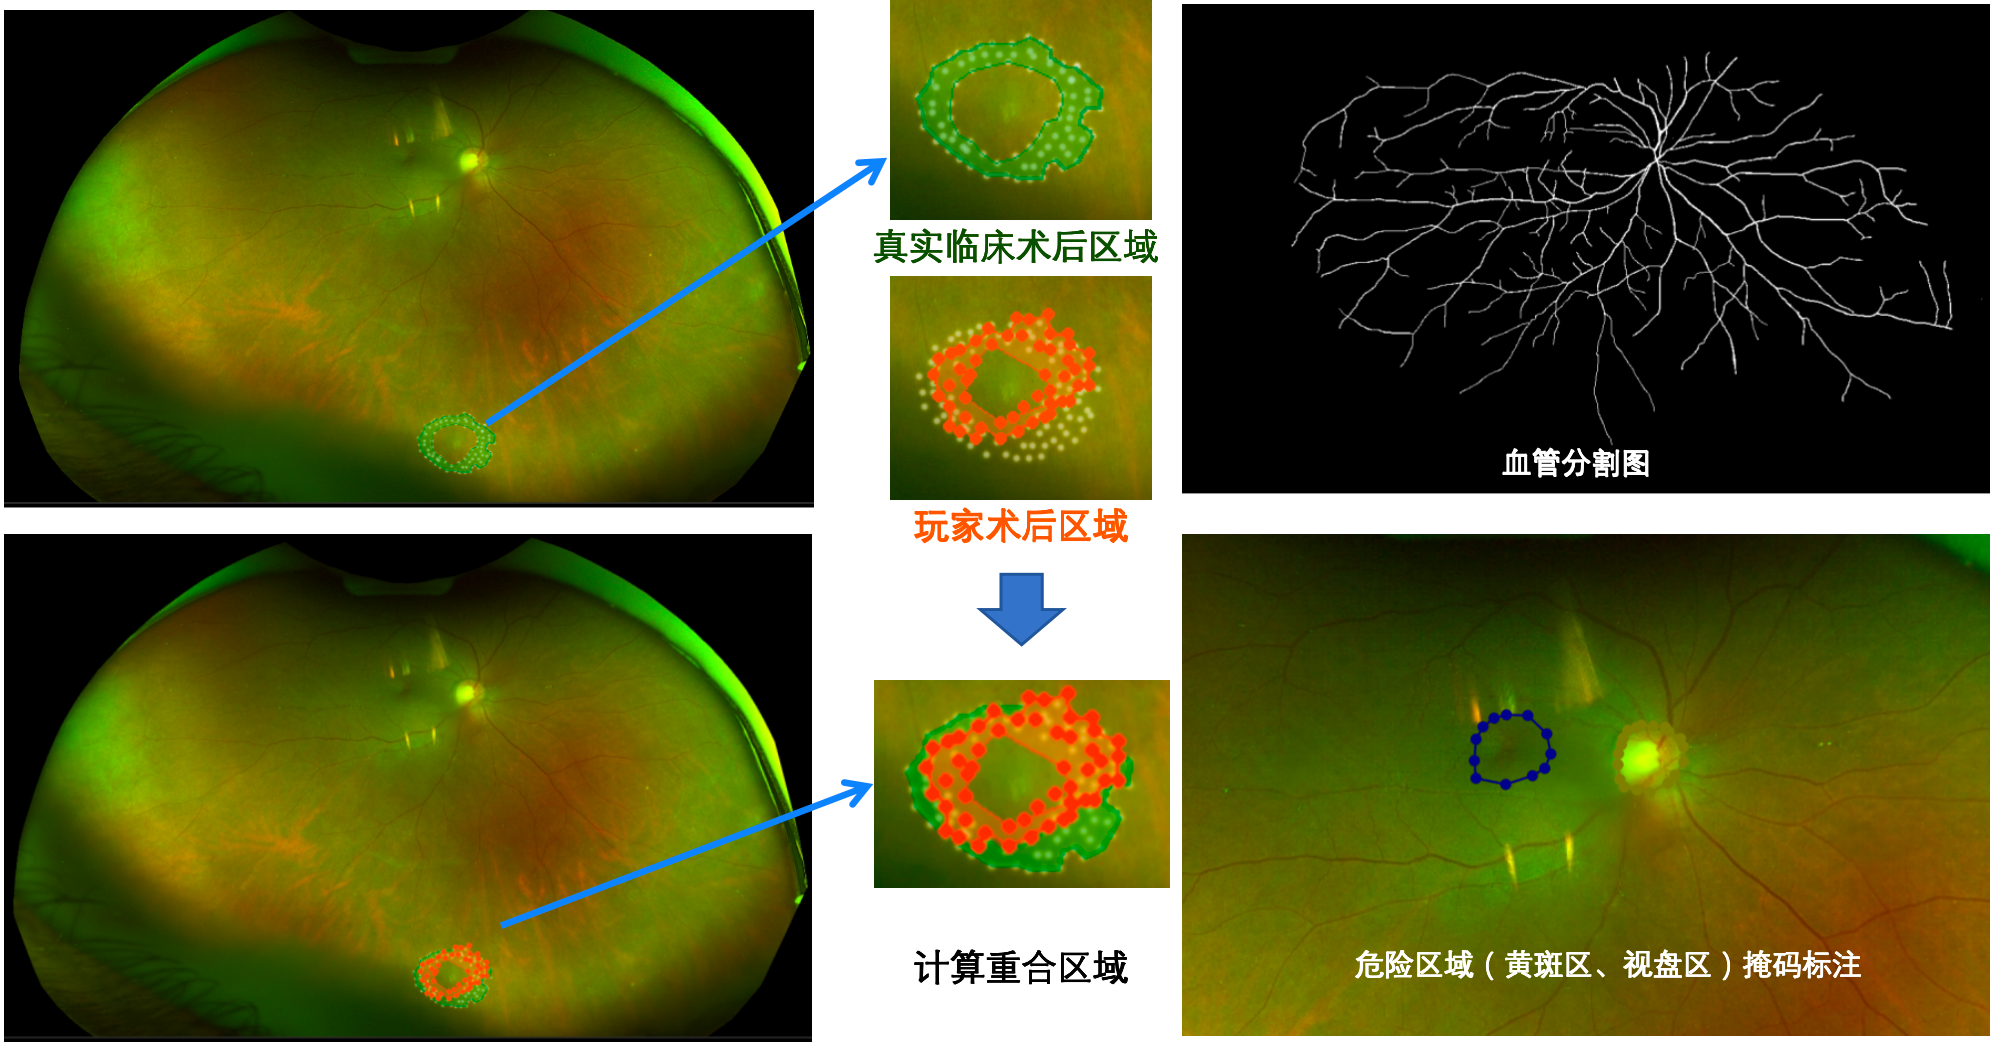
\includegraphics[width=1\linewidth]{score.png}
    \caption{智能评价系统评分结果与可视化反馈示例}
    \label{fig:smart_eval_score}
\end{figure}

\paragraph{LLM 教学复盘链路}
在教学复盘层，系统将“结构化评分结果 + 题目病历文本 + 专家知识库片段”组合后输入大语言模型，生成面向训练的自然语言反馈报告（优点、缺点、改进建议）。由于前置评分已提供可量化证据，LLM 的职责从“主观打分”转为“基于证据的教学表达”，从而提升反馈一致性与可解释性。

\subsubsection{后端开发}

\paragraph{分层架构与接口设计}
后端采用了分层架构，核心模块包括用户注册认证、关卡数据管理、会话提交、智能评分与静态资源服务。所有业务表都统一在了 PostgreSQL 的 同一schema 下，目前接口涵盖了玩家注册、登录、登出、关卡详情查询、评估、会话提交（支持 JSON 和 multipart/form-data）等，保证了数据一致性和接口的可扩展性。 

\paragraph{多模态数据处理与存储}
后端支持处理和存储多种数据类型，包括结构化 JSON（如玩家操作日志、关卡参数）、图片（如术前/术后图、评估可视化结果）、文本等。所有上传和生成的文件统一存储在 data/sessions/ 目录下，并通过数据库记录元数据，便于后续检索和管理。
\paragraph{智能评分与 Python 引擎集成}
通过 Java 的 ProcessBuilder 动态调用 Python 评分脚本，实现自动化的手术结果评估。后端负责参数准备、输入输出文件管理、超时控制和异常处理，确保评分流程的稳定性和可追溯性。评估结果 JSON 直接返回前端，并与相关文件路径一同写入数据库。
\paragraph{静态文件与可视化资源统一访问}
实现了统一的静态文件访问接口（/api/file），前端可通过标准 URL 直接访问评估报告、图片等资源。路径处理采用相对于程序运行时“当前工作目录”的相对路径方式，兼容不同操作系统和部署环境，避免路径混乱和权限问题。
\paragraph{安全性与健壮性设计}
路径访问严格白名单校验，防止任意文件读取。所有接口均有相应的参数校验和异常处理，保证服务的健壮性。数据库操作采用预编译语句，防止 SQL 注入。
\paragraph{易用性与可移植性}
支持通过环境变量灵活配置数据库连接参数。评估脚本路径、Python 解释器等均可通过参数指定，便于跨平台部署和本地/服务器环境切换。文件上传接口支持多种字段别名，兼容不同前端实现


\section{期中进展与阶段性成果}
\begin{enumerate}
    \item \textbf{交互场景与逻辑实现}：完成游戏开始菜单、诊疗室、游戏内手机以及术后图鉴式图文反馈报告的场景搭建。具体而言，开始菜单实现了开发致谢与设置的子功能面板，以及实现简单的存档系统，提供游戏继续或重新开始的启动接口。诊疗室作为游戏场景切换与功能呼出的中枢场景，支持玩家于其中位移，与任务相关仪器/物品进行交互。游戏内手机与术后图文反馈报告，均已实现场景搭建与布局设计，对象封装良好，待游戏运行时，从后端接受数据进行对象创建与属性绑定。
    \item \textbf{动作逻辑构建}：为增强游戏的视觉体验，在玩家与诊疗室移动，以及与仪器交互的转场过程中加入角色动作。其中交互动作额外添加背景淡化效果，增加转场视觉表现。实现了包括角色站立、移动、存取文档、与电脑交互以及与光凝仪器交互的五个动画构建，通过设定关键帧的方式，静态调整每帧用时。截图可见逐帧切片。在Unity里构建了角色的动作逻辑，绑定了动作触发条件，设置前后延迟时间、抗打断或过渡时间。
    \begin{figure}
        \centering
        \includegraphics[width=1\linewidth]{Actions.png}
        \caption{角色行为逻辑与动作逐帧切片}
        \label{fig:enter-label}
    \end{figure}
    \item \textbf{仿真功能实现}：实现了基于物理方程的多波长热损伤分级模型，支持从轻微凝固到组织焦化的四级病变连续模拟。开发了多层高斯过程化渲染算法，结合局部背景采样逼真还原光斑视觉特征。同时也完成了初步Unity界面的开发，能够支持基本的玩家交互操作和导出手术数据。
    \item \textbf{智能评价模块实现}：规定了题库样本的数据规范和游戏流程的数据结构。实现了基于位置与范围、强度与能量、密度与均匀度三个维度的评分计算模块，打通了从手术仿真层获取玩家操作日志和题目答案、计算玩家得分、玩家得分输入大模型、大模型输出教学反馈报告、在游戏前端实时展示反馈报告的全流程链路。能够支持玩家在游戏结束后实时地获取教学反馈。
    \begin{figure}[h]
        \centering
        \includegraphics[width=1\linewidth]{f4.png}
        \caption{进度展示-Unity界面}
        \label{fig:placeholder}
    \end{figure}
    \item \textbf{翻译实验验证}：验证了 Reverse Residual 方案在术后图像外观重建上的可行性。
    \item \textbf{后端服务搭建}：实现基于 PostgreSQL 的用户管理系统和基于http的接口并集成 Python 评分引擎。
\end{enumerate}








\section{遇到的挑战与解决方案}
\begin{itemize}
    \item \textbf{数据瓶颈}：目前缺乏完全配对的高质量数据（约30例），且大部分为伪彩图。后续会开发专用标注工具补齐光斑位置标注；
    \item \textbf{图像对齐问题}：局部裁剪区域在配对训练时对齐度不足，影响了可视化效果。后续会引入基于血管关键点的裁剪技术提升局部 Patch 的对齐精度。
    \item \textbf{手术仿真}：手术仿真中并没有考虑眼底球形结构对于激光强度的影响，矩阵发射模式也未考虑矩阵中不同位置的激光强度变化，需要重新建模。同时光斑的形状也还需要和医生进行进一步的确认。另一个问题是目前的仿真缺乏裂隙灯调焦模拟的关键步骤，之后需要添加。
    \item \textbf{线上问诊拟真度低}：当前版本中，右栏聊天内容仍主要直接来自医院文本数据，口语化模拟程度有限，且玩家尚无法在该界面中直接完成病症选择与判断提交。后续我们计划通过大模型接入或离线病例语料库构建的方式，对医院文本信息进行生活化改写，并引入“病征无关信息混合”机制，以增强问诊环节的真实性、复杂度与训练价值，从而进一步提升玩家在光凝相关疾病诊断中的信息甄别能力。
    \item \textbf{反馈报告布局与篇幅限制}：该页面目前仍存在明显局限。首先，现有布局较适合单病灶或病灶数量较少的病例，对于后续复杂病症中的多病灶情况，当前截图区域与对比面板很可能难以兼顾信息完整性与阅读效率。其次，分析报告的篇幅目前经过有意压缩，以避免玩家面对过长文本产生厌读心理，但随着病症复杂度增加，现有中等篇幅可能不足以提供充分而有效的复盘信息。对此，后续仍需围绕多病灶信息组织、报告结构压缩与重点突出机制持续优化。
    \item \textbf{诊所中枢场景留存较大空余，及状态信息提示不足}：诊所中枢场景在视觉布局上仍预留了较大空间。当前版本中，场景上下区域存在相对明显的空余，这一方面意味着现有信息密度尚未饱和，另一方面也为后续加入状态提示 UI、患者到访动画、经营状态反馈及额外娱乐性内容提供了结构性留白。以当前规划看，当患者来到诊所进行手术时，可进一步加入角色入场、步行至仪器前等动画表现，以增强诊所作为“经营空间”的动态感与沉浸感。
\end{itemize}

\section{后续计划}


\begin{table}[H]
    \centering
    \caption{项目任务与具体时间节点分配表}
    \label{tab:task_matrix}
    % \textwidth 表示表格总宽度等于页面文本宽度
    % c 表示第一列居中；X 表示后面的列自动平分宽度且支持内部文字换行
    % >{\raggedright\arraybackslash} 是为了让 X 列里的文字左对齐，阅读更舒适
    \begin{tabularx}{\textwidth}{c *{3}{>{\raggedright\arraybackslash}X}} 
        \toprule
        % 第一行：成员名字纵向合并2行；时间节点横跨后面的3个大列
        \multirow{2}{*}{\textbf{成员}} & \multicolumn{3}{c}{\textbf{时间节点}} \\
        \cmidrule(lr){2-4} 
        
        % 第二行：具体的两周一次的时间节点（共3列）
        & \textbf{第9\textendash 10周} & \textbf{第11\textendash 12周} & \textbf{第13\textendash 14周} \\
        \midrule
        
        % 正式成员填入任务。如果某周没任务，就直接留空即可（保留 & 符号）
        冯俊铭 & 整理医院的新数据，制作并完善真实数据题库 & 收集、整理相关手术专业知识文档，构建专家知识库辅助大语言模型生成报告 & 收集玩家和专家的反馈，微调模型架构 \\ 
        吴嘉淇 & 优化手术操作界面UI，和游戏整体风格对齐并接入主场景& 实现调焦功能的模拟并尝试模拟眼底的球形结构以及该结构对光斑效果造成的影响& \\ 
        林鸿渝 & 诊疗室状态提示添加，视听效果丰富，游戏内功能查漏补缺 & 使用后端大模型API实现更拟真的线上问诊 & 项目整合，查漏补缺\\ 
        陈俊希 & 完善后端接口，增加会话历史查询、关卡管理等功能& 支持多用户并发和权限管理，完善用户体验  & 整体调试，修补漏洞\\ 
        吴雨潼 & 完成新标注工具的开发，手动根据血管关键点裁剪出新的配对数据& 对标注流程进行自动化或尽量减少需要手工标注的部分，初步训练模型 &  \\ 
        史卓然 & & &  \\ 
        
        \midrule
        % 低年级学弟的任务可以分配在不同周
        学弟学妹 & 对医院原始数据标注血管分割图和危险区  & 四个指导性小游戏设计开发，对应四种不同眼底光凝术病症策略教学 &  \\ 
        
        \bottomrule
    \end{tabularx}
\end{table}


\section{参考文献}
\begin{itemize}
    \item [1] Jain A, Blumenkranz MS, Paulus Y, et al. Effect of pulse duration on size and character of the lesion in retinal photocoagulation. Arch Ophthalmol. 2008;126(1):78-85.
    \item [2] 《Baba is you》, Hempuli, 2019.
    \item [3] 《Microsoft Flight Simulator》, Asobo Studio, 2020.

\end{itemize}

\vspace{1em}
\templaterule
\vspace{1em}

\noindent{\zihao{3}\bfseries 个人部分：课程建议与项目心得}\par
\vspace{0.6em}

在本次项目中，我主要负责智能评价系统（模型2）相关工作，包括评分规则落地、评估引擎实现及与后端/前端的联调。从结果来看，我最大的体会是：教学反馈系统的核心不是“把分数算出来”，而是“把可执行的改进建议讲清楚”。因此我们将评分链路拆成了可验证的三个层次：先做结构化指标计算（位置覆盖、能量参数、点位均匀性），再做安全约束判定（黄斑/视盘红线与血管惩罚），最后再将结构化证据输入 LLM 生成自然语言复盘。这样做的好处是，每一条反馈都有来源字段和可视化证据支撑，避免了黑盒式评价。

具体到工程实践，我感受到“鲁棒性”比“单次精度”更重要。真实联调时，题库标注、玩家日志和测试样本的格式并不总是统一，如果没有输入标准化和异常兜底，系统就会频繁中断，无法支持训练闭环。基于这一问题，我在评估器中加入了多格式兼容、凹包重建失败回退、危险区多来源检测等机制，优先保证流程稳定可运行，再逐步优化评分细节。

在本次项目中我作为组长，要协调全组成员完成一个系统性的工程项目，在过程中我学到了很多团队协作的经验，包括如何制定计划、如何分配任务、如何协调进度、如何解决问题等。同时，我也学到了很多项目管理方面的知识，包括如何制定项目计划、如何分配任务、如何协调进度、如何解决问题等。 好在队友们都十分配合，能够及时完成任务，并且能够及时解决问题，使得项目能够顺利进行。

前半学期的课程中，我学到了很多关于多媒体信息处理方面的基础知识，包括图像处理、视频处理、音频处理等。在后半学期的课程中，如果有机会我希望加入更多的实机演示和动画效果，以及一些比较常见好理解的样例，这样在学习相应算法的时候可以帮助我们更好地理解算法的运行过程和结果。
\end{document}
